\documentclass[12pt]{article}
\usepackage{geometry}                % See geometry.pdf to learn the layout options. There are lots.
\geometry{letterpaper}                   % ... or a4paper or a5paper or ... 
\usepackage{graphicx}
\usepackage{amssymb}
\usepackage{amsthm}
\usepackage{epstopdf}
\usepackage[utf8]{inputenc}
\usepackage[usenames,dvipsnames]{color}
\usepackage[table]{xcolor}
\usepackage{hyperref}
\DeclareGraphicsRule{.tif}{png}{.png}{`convert #1 `dirname #1`/`basename #1 .tif`.png}

\theoremstyle{definition}
\newtheorem{example}{Example}

\newcommand{\projectname}{Smart Shopping List}
\newcommand{\productname}{Smart Shopping List}
\newcommand{\projectleader}{A. Walliser}
\newcommand{\documentstatus}{In process}
%\newcommand{\documentstatus}{Submitted}
%\newcommand{\documentstatus}{Released}
\newcommand{\version}{V. 1.0}

\begin{document}
\begin{titlepage}
\begin{flushright}

\includegraphics[scale=.5]{htlleondinglogo.png}\\
\end{flushright}

\vspace{10em}

\begin{center}
{\Huge System Specification} \\[3em]
{\LARGE \productname} \\[3em]
\end{center}

\begin{flushleft}
\begin{tabular}{|l|l|}
\hline
Project Name & \projectname \\ \hline
Project Leader & \projectleader \\ \hline
Document state & \documentstatus \\ \hline
Version & \version \\ \hline
\end{tabular}
\end{flushleft}

\end{titlepage}
\section*{Revisions}
\begin{tabular}{|l|l|l|}
\hline
\cellcolor[gray]{0.5}\textcolor{white}{Date} & \cellcolor[gray]{0.5}\textcolor{white}{Author} & \cellcolor[gray]{0.5}\textcolor{white}{Change} \\ \hline
November 29, 2018&C. Wagner/A. Walliser&First version \\ \hline
\end{tabular}
\pagebreak

\tableofcontents
\pagebreak

\section{Initial Situation and Goal}

\subsection{Initial Situation}

Members of a typical household must go shopping for groceries at least once a week. A lot of households use grocery lists to organise that process. Problems that could occur are that the grocery list gets lost or if the list is in use nobody else can add shopping items to the list. It also could happen that multiple lists get written because of miscommunication between the members of a household.

Furthermore things get more complex when the combination of recipe books and grocery lists is considered. The items found in different recipe books have to be manually transferred to the shopping list. 

These processes could be simplified by using a grocery list app.

\subsubsection{Application Domain}
Most people write a shopping list before they go shopping. When one member of a household goes shopping they only buy the products they wrote down. To not forget a product they have to communicate with every member of the household and ask them which items they want. Furthermore the items are written down in the order the writer is thinking of it, but in the store they want the items to be sorted according to the departments they belong to. 
\subsubsection{Glossary}

\subsubsection{Model of the Application Domain}


\subsubsection{Overview of the Business Processes}

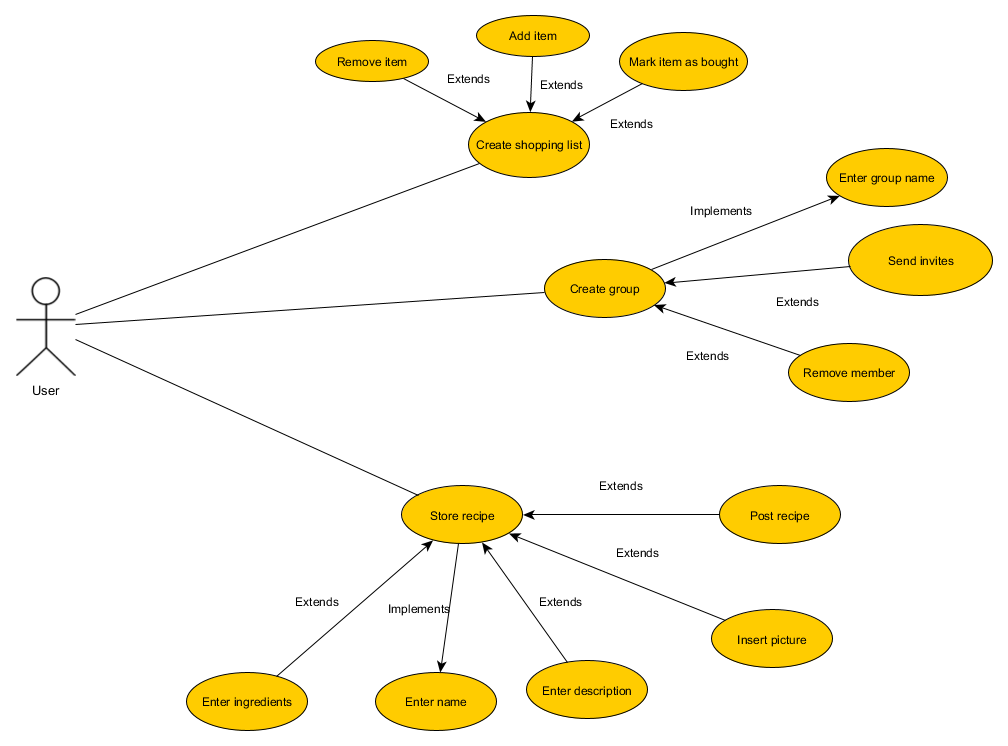
\includegraphics[scale=.5]{UseCase.png}

\subsection{Goal Definition}

\pagebreak

\section{Functional Requirements}

\subsection{Use-Case Diagrams}

\subsection{Use Case Store Recipe}

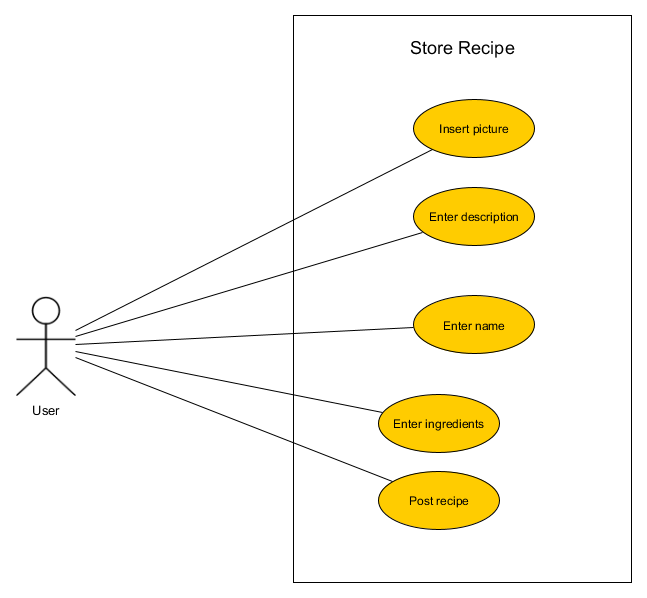
\includegraphics[scale=.5]{UseCaseStoreRecipe.png}\\

\subsubsection{Characteristic Information}

\begin{tabular}{|l|l|}
\hline
Goal & Creates a recipe that is added to the users recipelist  \\ \hline
Precondition & none \\ \hline
Postcondition & New recipe in the recipelist \\ \hline
Involved User & The user who wants to create a recipe \\ \hline
Triggering Event & Event is triggered by the user \\ \hline
\end{tabular}

\subsection{Use Case Create Group}

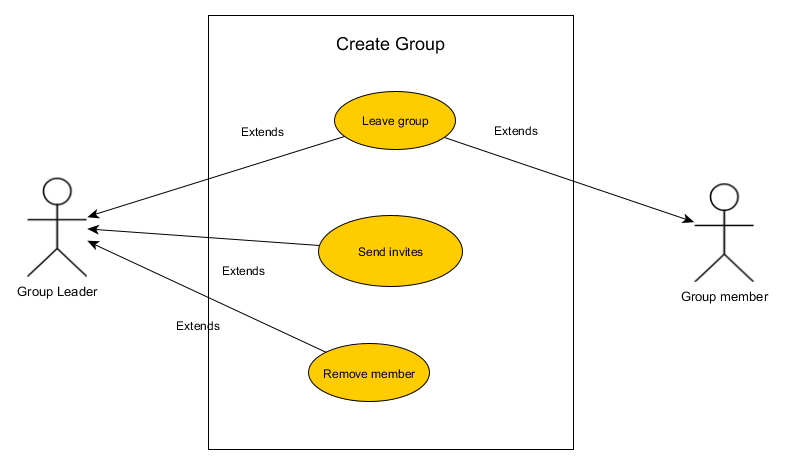
\includegraphics[scale=.5]{UseCaseCreateGroup.png}\\



\subsubsection{Characteristic Information}

\begin{tabular}{|l|l|}
\hline
Goal &  Create a group with the creators items and categories\\ \hline
Precondition & none\\ \hline
Postcondition & New group in the users list of groups which contains the creators items and categories \\ \hline
Involved User &  \\ \hline
Triggering Event & Event is triggered by the user \\ \hline
\end{tabular}

\subsection{Use Case Create Shoppinglist}

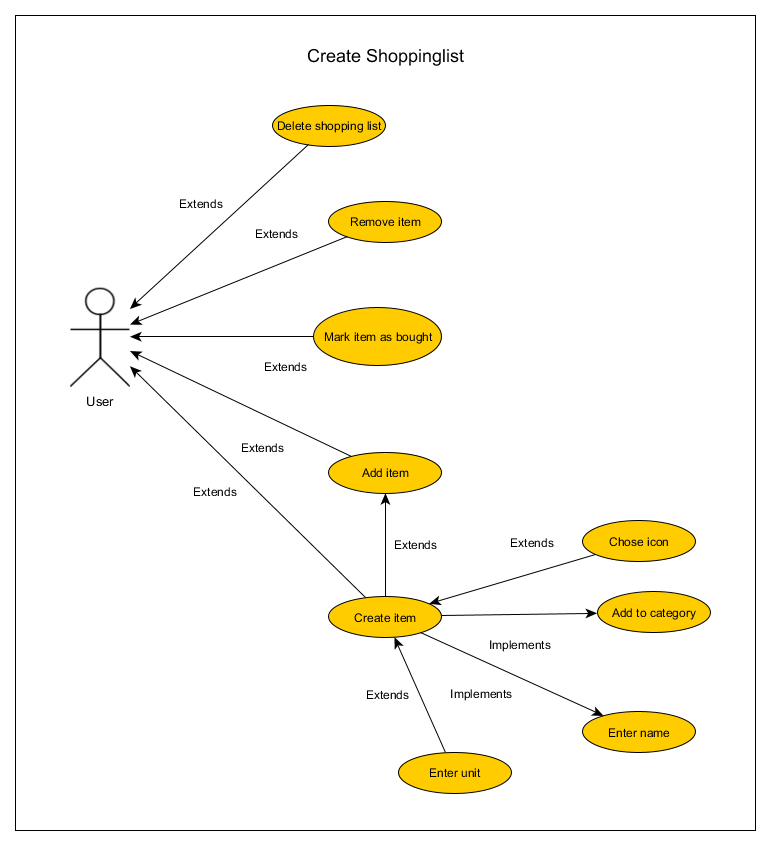
\includegraphics[scale=.5]{UseCaseCreateShoppinglist.png}\\


\subsubsection{Characteristic Information}

\begin{tabular}{|l|l|}
\hline
Goal &  \\ \hline
Precondition &  \\ \hline
Postcondition &  \\ \hline
Involved User &  \\ \hline
Triggering Event &  \\ \hline
\end{tabular}


\subsubsection{GUI to call the use case}

\begin{tabular}{|l|l|}
\hline
Input field & Valid inputs \\ \hline
 &  \\ \hline
\end{tabular}

\subsubsection{Scenario for the standard use}

\begin{tabular}{|l|l|l|}
\hline
Step & User & Activity \\ \hline
 & & \\ \hline
\end{tabular}

\subsubsection{GUIs for the standard use}

\begin{tabular}{|l|l|}
\hline
Input field & Valid inputs \\ \hline
 &  \\ \hline
\end{tabular}

\subsubsection{Scenarios for non-standard uses}

\begin{tabular}{|l|l|l|}
\hline
Step & User & Activity \\ \hline
 & & \\ \hline
\end{tabular}

\subsubsection{GUIs for the non-standard uses}

\begin{tabular}{|l|l|}
\hline
Input field & Valid inputs \\ \hline
 &  \\ \hline
\end{tabular}

\subsubsection{Workflow}

\subsubsection{Open Points}

\pagebreak

\section{Non-functional Requirements}

\pagebreak

\section{Quantity Structure}

\pagebreak

\section{System Architecture and Interfaces}

\pagebreak

\section{Acceptance Criteria}

\pagebreak

\section{Acceptance Criteria}

\pagebreak

\section{References}

\pagebreak

\section{List of Figures}

\pagebreak

\end{document}  